
\chapter*{\begin{center}
{\Large \bfseries ABSTRACT}
\end{center}}
\noindent
\begin{figure}[H]
\centering
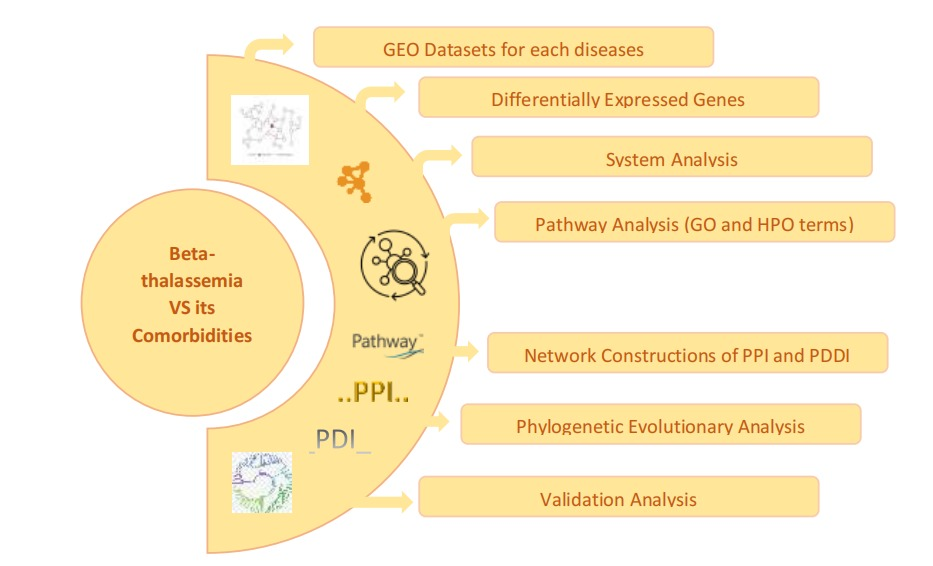
\includegraphics[width=15cm]{logos/abstract_fig.jpg}
\end{figure}

\noindent
Beta-thalassemia (BT), a genetic blood anomaly brought on by abnormalities in the HBB gene that occurs when beta-globin chain production is reduced or absent in blood. It is a major worldwide health issue because of its complicated clinical management and lifetime reliance on blood transfusions. Some recent evidence highlights that beta-thalassemia is associated with several comorbidities, including endocrine diseases involving polycystic ovarian syndrome (PCOS), hypothyroidism, hypogonadism and type 2 diabetes (T2D) and cardiovascular diseases involving arrhythmogenic cardiomyopathy (ACM) and arrhythmia. These comorbidities may share common molecular mechanisms with beta-thalassemia that potentially exacerbate disease severity and treatment complications. In this study, a computational approach was applied to evaluate the genetic relationships between beta-thalassemia and its associated comorbidities using microarray and mRNA datasets that are publicly available in NCBI. Genetic profiling was constructed to identify the common matching genes and built disease-gene networks (DGNs) of matching genes. It also visualized a heatmap to present patterns of gene expressions. We also explored multiple bioinformatics analysis including pathways, gene ontology, protein-protein interaction (PPI) and protein-drug interaction (PDI) that strongly indicate their correlation. A validation network was created to verify our selected comorbidity and then phylogenetic analysis was performed for all diseases to determine their evolutionary relationships. This study found that beta-thalassemia shares 13, 165, 13, 14, 11 and 44 significantly expressed genes with hypothyroidism, hypogonadism, PCOS, T2D, ACM and arrhythmia respectively. The outcomes of this study may help in integrative medical approaches and enhance a significant understanding of genetic and molecular structure of comorbidities in beta-thalassemia by providing valuable insights.

\vspace{0.5cm}
 
\textbf{Keywords}: Beta-thalassemia, comorbidities, genetic profiling, endocrine diseases, cardiac diseases, arrhythmogenic cardiomyopathy, pathway analysis, ontology, phylogenetic analysis.

\clearpage
